\let\negmedspace\undefined
\let\negthickspace\undefined
\documentclass[journal]{IEEEtran}
\usepackage[a5paper, margin=10mm, onecolumn]{geometry}
%\usepackage{lmodern} % Ensure lmodern is loaded for pdflatex
\usepackage{tfrupee} % Include tfrupee package

\setlength{\headheight}{1cm} % Set the height of the header box
\setlength{\headsep}{0mm}     % Set the distance between the header box and the top of the text

\usepackage{gvv-book}
\usepackage{gvv}
\usepackage{cite}
\usepackage{amsmath,amssymb,amsfonts,amsthm}
\usepackage{algorithmic}
\usepackage{graphicx}
\usepackage{textcomp}
\usepackage{xcolor}
\usepackage{txfonts}
\usepackage{listings}
\usepackage{enumitem}
\usepackage{mathtools}
\usepackage{gensymb}
\usepackage{comment}
\usepackage[breaklinks=true]{hyperref}
\usepackage{tkz-euclide} 
\usepackage{listings}
% \usepackage{gvv}                                        
\def\inputGnumericTable{}                                 
\usepackage[latin1]{inputenc}                                
\usepackage{color}                                            
\usepackage{array}                                            
\usepackage{longtable}                                       
\usepackage{calc}                                             
\usepackage{multirow}                                         
\usepackage{hhline}                                           
\usepackage{ifthen}                                           
\usepackage{lscape}
\begin{document}

\bibliographystyle{IEEEtran}
\vspace{3cm}

\title{10.4.3.3.2}
\author{EE24BTECH11012 - Bhavanisankar G S}
% \maketitle
% \newpage
% \bigskip
{\let\newpage\relax\maketitle}

\renewcommand{\thefigure}{\theenumi}
\renewcommand{\thetable}{\theenumi}
\setlength{\intextsep}{10pt} % Space between text and floats


\numberwithin{equation}{enumi}
\numberwithin{figure}{enumi}
\renewcommand{\thetable}{\theenumi}

\textbf{QUESTION} : \\
Find the roots of the quadratic equation, $\frac{1}{x+4} - \frac{1}{x-7} = \frac{11}{30}, x \neq -4, 7$. \\
\textbf{SOLUTION} : \\
\begin{enumerate}
	\item \textbf{QUADRATIC FORMULA} : \\
	Consider an equation, 
	\begin{align}
		ax^2 + bx + c &= 0 \\
	        x^2 + \frac{b}{a} x + \frac{c}{a} &= 0 \label{eq:qe} \\
		x^2 + 2 \frac{b}{2a} x + \frac{b^2}{4a^2} - \frac{b^2}{4a^2} + \frac{c}{a} &= 0 \\
		\brak{x + \frac{b}{2a}}^2 + \brak{\frac{4ac - b^2}{4a^2}} &= 0 \\
		\brak{x + \frac{b}{2a}} &= \frac{\sqrt{b^2 - 4ac}}{2a} \\
		x &= \frac{-b \pm \sqrt{b^2 - 4ac}}{2a}
	\end{align}
	which is the quadratic formula. \\
Given equation, 
\begin{align}
	\frac{1}{x+4} - \frac{1}{x-7} &= \frac{11}{30}, x \neq -4, 7 \\
	\frac{-11}{\brak{x+4}{x-7}} &= \frac{11}{30} \\
	\implies x^2 - 3x + 2 &= 0 \\
	\implies x &= 1 \\
	x &= 2
\end{align}
	\item \textbf{EIGENVALUE APPROACH} : \\
	Consider the equation, \eqref{eq:qe}. It can be rearranged as
	\begin{align}
		\lambda ^2 + \frac{b}{a} \lambda + \frac{c}{a} &= 0 \\
		\lambda \brak{\lambda + \frac{b}{a}} + \frac{c}{a} &= 0 \\
		-\lambda \brak{-\lambda - \frac{b}{a}} - (-1) \frac{c}{a} &= 0
	\end{align}
	This can be considered equivalent to the determinant of the matrix, 
	\begin{align}
		\myvec{-\lambda & 1 \\ -\frac{c}{a} & \frac{-b}{a} - \lambda} \label{eq:matrix}
	\end{align}
	Clearly, it can be seen that the eigenvalues of the matrix 
	\begin{align}
		\myvec{0 & 1 \\ \frac{-c}{a} & \frac{-b}{a}} \label{eq:cmat}
	\end{align}
	are the roots of the required quadratic equation. This matrix, \eqref{eq:cmat} is called the \textbf{Companion matrix} \brak{\vec{C}}. \\
	For the given question, 
	\begin{align}
		\vec{C} &= \myvec{0 & 1 \\ -2 & 3}
	\end{align}
	\textbf{QR ALGORITHM} :
	Eigenvalues of the companion matrix can be found using QR algorithm. Using the Gram-Schmidt orthogonalization, the matrix $\vec{C}$ can be factorized into
	\begin{align}
		\vec{C} &= \vec{Q} \vec{R}
	\end{align}
	where, 
	\begin{align}
		\vec{Q} &= Orthonormal matrix \\
		\vec{R} &= Upper triangular matrix
	\end{align}
	This process can be continues as
	\begin{align}
		\vec{C_{k}} &= \vec{Q_{k}} \vec{R_{k}} \\
		\vec{C_{k+1}} &= \vec{R_{k}} \vec{Q_{k}}
	\end{align}
	As $k \to \infty$, the diagonal elements of $\vec{Q_{k}}$ converge to the eigenvalues of the matrix.
	It can be seen that eigenvalues are 1 and 2.
	\item \textbf{Newton-Raphson method} : \\
		We have, 
		\begin{align}
			x_{n+1} &= x_{n} - \frac{f(x_{n})}{f^{\prime}(x_{n})}	\\
			x_{n+1} &= x_{n} - \frac{x_{n}^2 - 3x_{n} + 2}{2 x_{n} - 3}
		\end{align}
		Iterating and updating the value of $x_{n}$, we can obtain the roots of the quadratic equation. \\
		The roots found using this method taking the initial guesses as 10 and 0 are 2.000000000905422 and 1.0000000022055868
 respectively.
 
\end{enumerate}
\begin{figure}[h]
\centering
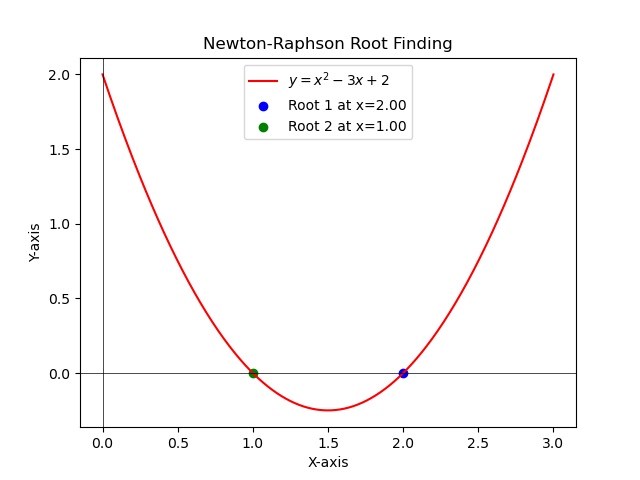
\includegraphics[width=\columnwidth]{figs/fig.png}
\caption{Plot of the given question.}
\label{fig:Plot1} 
\end{figure}
\end{document}
